\subsection{Mapping properties of the exponential}
We know that the map $w = e^z$ is periodic with period $2\pi i$. By noting that $e^{x + iy} = e^x(\cos(y) + i \sin(y))$ we see that horizontal lines are mapped to rays (approaching the origin) and vertical lines are mapped to circles (centered at the origin). 

We can force $e^z$ to be injective by restricting its domain. In particular the map is injective on domains of the form $\{z \in \C : a <  \Im(z) < b\}$ with $b - a \leq 2\pi$. If $b - a = 2\pi$ then the image of this strip is $\C \setminus [0, \infty)$. If $b - a < 2\pi$ then the image of the strip is a sector of the plane (recall horizontal lines are mapped to rays). 

We can do a similar exercise with $\log$ but first we would like to make it better behaved by considering it as a map from some appropriate covering space, i.e. Riemann surface. As before, we will take $X$ to be the graph of the exponential. To be precise, $X := \{(z, w) \in \C^2 : z = e^w\}$. Then of course the $\log$ function is simply a mapping onto the second coordinate. Note in this case that small neighbourhoods in $\C$ have countably many copies of themselves in $X$, the Riemann surface for $\log$. Thus $X$ forms a spiral of sorts.

The $\log$ function then allows us to invert the transformations above. For example, we can transform $\C \setminus [0, \infty)$ to a horizontal strip between $\Im(z) = 2\pi i$ and $\Im(z) = 0$. 

\section{Analytic Functions}
\begin{definition}[Analytic functions]
A function $f$ is analytic in an open set $\Omega$ if it has a convergent power series representation at every point in $\Omega$. That is to say, $f$ is analytic in $\Omega$ if for any $z_0 \in \Omega$, there is a convergent power series $\sum_{n = 0}^\infty a_n (z - z_0)^n$ so that $f(z) = \sum_{n = 0}^\infty a_n (z - z_0)^n$ in the open disk $\abs{z - z_0} < r$ for some $r$ less than or equal to the radius of convergence for the power series.
\end{definition}

One of the nice things about analytic functions is that it can sometimes be easier to do operations using the power series representation. For example, given an analytic function $f$, we can easily find its primitive $g$ since if 
$$ f(z) = \sum_{n = 0}^\infty a_n (z - z_0)^n $$
then
$$ g(z) = \sum_{n =0}^\infty \frac{a_n}{n + 1}(z - z_0)^{n+1} $$
Moreover we know the two series have the same radius of convergence (see \autoref{thm:radius-of-conv}). 

The first thing we want to verify that functions given by power series are indeed analytic (at least within their radius of convergence)
\begin{proposition}
If $f(z) = \sum_{n = 0}^\infty a_n z^n$ has a convergent power series with radius of convergence $R$ then $f(z)$ is analytic in the open disk $\abs{z} < R$.
\end{proposition}
\begin{remark}
Above we assume that the series expansion is centered at the origin. This is mostly to make the computations slightly easier and of course the theorem holds more generally for series centered at any point.
\end{remark}
\begin{proof}
We will show that for any $\abs{z_0} < R$, $f$ has a convergent power series centered at $z_0$ and that the convergence is uniform and absolute in the closed disk $\abs{z - z_0} \leq r$ for any $r < R - \abs{z_0}$. We see that
\begin{align*}
    f(z) &= \sum_{n = 0}^\infty a_n (z_0 + (z - z_0))^n\\
    &= \sum_{n = 0}^\infty a_n \sum_{k = 0}^n \binom{n}{k} z_0^{n - k} (z - z_0)^k 
\end{align*}
We know that $z$ above is in the radius of convergence for the series centered at the origin (this is a consequence of the triangle inequality since $\abs{z} \leq \abs{z - z_0} + \abs{z_0} < R - \abs{z_0} + \abs{z_0} = R$). Convergence is absolute within the radius of convergence (again, see \autoref{thm:radius-of-conv}). In particular this means that we can rearrange the order of summation without changing its value. Doing this above, allows us to conclude that
$$ f(z) = \sum_{k = 0}^\infty \left( \sum_{n = k}^\infty a_n \binom{n}{k} z_0^{n - k} \right) (z - z_0)^k $$
\end{proof}

\subsection{Principle of Analytic Continuation}
\begin{theorem}
Let $f(z)$ be analytic in a domain (connected open set) $\Omega$ and $z_0 \in \Omega$. The following are equivalent:
\begin{enumerate}
    \item $f^{(n)}(z_0) = 0$ for $n = 0, 1, \dots$
    \item $f$ is identically 0 in a neighbourhood of $z_0$
    \item $f$ is 0 in $\Omega$
\end{enumerate}
\end{theorem}
\begin{proof}
$(3) \Rightarrow (1)$ is trivial. $(1) \Rightarrow (2)$ follows immediately from the power series representation of $f$ at $z_0$ (recall Taylor's theorem). The only direction we need to work on then is $(2) \Rightarrow (3)$.

Let $\Omega' = \{z \in \Omega : f \equiv 0 \text{ in a neighbourhood of $z$ in } \Omega\}$. We know that $\Omega'$ is non-empty sine $z_0$ is in $\Omega'$. It is also immediate from the definition that $\Omega'$ is open. What we want to show then is that $\Omega'$ is closed. Let $z \in \ol{\Omega'}$ (closure of $\Omega'$). Continuity of derivatives implies that $f^{(n)}(z) = 0$ for all $n \in \N$ ($z$ can be expressed as the limit of points each of which has 0 derivatives). Therefore, by $(1) \Rightarrow (2)$ we know that $f$ is identically 0 in a neighbourhood of $z$ implying that $z \in \Omega'$. since $\Omega' = \ol{\Omega'}$ we conclude that $\Omega'$ is closed. Connected of $\Omega$ implies that $\Omega' = \Omega$.
\end{proof}

The reason that the above forms the principle of analytic continuation is due to the following corollary.
\begin{corollary}
If $f, g$ are analytic in a domain $\Omega$ and $f = g$ in a neighbourhood of some point, then $f = g$ in $\Omega$.
\end{corollary}
This means that if an analytic function can be continued, the continuation is unique. Another corollary of the theorem is that it gives the ring of analytic function on $\Omega$ a nice algebraic structure.
\begin{corollary}
The ring of analytic function $\mathscr{A}(\Omega)$ on $\Omega$ form an integral domain.
\end{corollary}
\begin{proof}
An integral domain is a ring where the product of two things being 0 implies that at least one of the things was 0. So suppose $fg = 0$ on $\Omega$ and $f \neq 0$. Then there is some $z_0 \in \Omega$ such that $f(z_0)$ is non-zero in a neighbourhood of $z_0$. Then $g$ must be 0 on this neighbourhood and therefore all of $\Omega$. 
\end{proof}

\subsection{Zeros and Poles of analytic functions}
Suppose $f$ is analytic in a neighbourhood of $z_0$. Then $f(z) = \sum_{n = 0}^\infty a_n (z - z_0)^n$ provided $z$ is close enough to $z_0$. Moreover, suppose $f(z_0) = 0$ but $f$ is not identically 0. In this case $f(z) \neq 0$ for $0 < \abs{z - z_0} < \epsilon$ for some $\epsilon > 0$. In other words the zeros of $f$ are isolate.

Let $k$ be the smallest integer such that $f^{(k)}(z_0) \neq 0$ (which is equivalent to saying $a_k \neq 0$). Then
$$ f(z) = (z - z_0)^k g(z) $$
where $g$ is analytic and $g(z_0) \neq 0$. Then we call $k$ the \textit{order} or \textit{multiplicity} of the zero $z_0$ of $f$. Given the above expression, we can define a coordinate change to make $f$ a very simple function, namely define $\zeta := (z - z_0)g(z)^{1/k}$. Then
$$ f(z(\zeta)) = \zeta^k $$

Now we consider the quotient of analytic functions. So consider $\frac{f(z)}{g(z)}$ where $g$ is not identically 0. If $g(z_0) \neq 0$ then $\frac{f(z)}{g(z)}$ is well-defined and analytic in a neighbourhood of $z_0$. Now suppose $g(z_0)$ is 0. Then we write $f(z) = (z - z_0)^k f_1(z)$ and $g(z) = (z - z_0)^l g_1(z)$ where as before we choose $k$ and $l$ so that $f_1(z_0)$ and $g_1(z_0)$ are non-zero. Then
$$ \frac{f(z)}{g(z)} = (z - z_0)^{k - l} \frac{f_1(z)}{g_1(z)} $$
If $k \geq l$ then $\frac{f}{g}$ extends to be analytic at $z_0$. Otherwise, if $k < l$ then $z_0$ is a pole of $\frac{f}{g}$ of order/multiplicity $l - k$. Note in this case
$$ \abs{\frac{f(z)}{g(z)}} \to \infty  $$
as $z \to \infty$. So $\frac{f}{g}$ makes sense as a function with values in Riemann sphere.

\begin{definition}[Meromorphic Function]
A \textit{meromorphic function} in an open set $\Omega$ is a function that is well-defined and analytic in the complement of a discrete set and expressible in a neighbourhood of \textit{any} point in $\Omega$ as a quotient of analytic functions $\displaystyle \frac{f}{g}$ where $g$ is not identically 0.
\end{definition}
Although meromorphic functions are slightly less well-behaved than analytic functions we will find that they provide the benefit of forming a field.

\section{Integration over curves}
Let $\Omega \subset \R^2$ be open. A curve in $\Omega$ is a map $\gamma: [a, b] \to \Omega$ which we usually take to be $C^1$ (or piecewise $C^1$). Sometimes we might write $\gamma(t) = (x(t), y(t))$ if we are interested in using its components.

We will be integrating 1-forms over curves. A 1-form $\omega$ can be written as 
$$\omega = Pdx + Qdy$$
where $P, Q$ are continuous functions on $\Omega$ (they might be real or complex-valued). Then
$$ \int_{\gamma} \omega = \int_a^b F(t) dt$$
where $F(t) = P(\gamma(t))x'(t) + Q(\gamma(t)) y'(t)$. This follows from the usual pullback formula since
$$ \gamma^*(Pdx + Qdy) = \gamma^*(P)\gamma^*(dx) + \gamma^*(Q)\gamma^*(dy) $$
We know that 
$$\gamma^*(P) = P \circ \gamma$$
and
$$ \gamma^*(dx) = d(\gamma^* x) = d(x \circ \gamma) = d(x(t)) = x'(t) $$

One thing we would like to know is that integration over a curve doesn't depend on how we parameterise the curve (loosely speaking integration should only depend on the image of the curve). Suppose $\delta(u) = \gamma(t(u))$ where $t: [c, d] \to [a, b]$ such that $t(c) = a$, $t(d) = b$ and $t' > 0$ in $(c, d)$ (the derivative condition is to ensure that orientation is preserved). Then we see that
$$ \delta^*\omega = (\gamma \circ t)^*\omega = t^*(\gamma^* \omega) = t^*(F du) = F(t(u)) t'(u) du $$
Then
$$ \int_{\delta} \omega = \int_{c}^d \delta^* \omega = \int_c^d F(t(u)) t'(u) du = \int_a^b F(t) dt = \int_\gamma \omega $$
using the usual integration by substitution formula. 

Therefore although $\displaystyle \int_\gamma \omega$ depends on $\omega$ and $\gamma$ (as an oriented curve) it does not depend on the parameterisation of $\gamma$. Of course if we flip orientations, we simply pick up a negative sign.\\

Suppose given an interval $[a, b]$ we partition it using $t_0 < t_1 < \dots < t_n$ where $t_0 = a$ and $t_n = b$. Then
$$ \int_\gamma \omega = \sum_{i = 1}^n \int_{\gamma_i} \omega \quad, \gamma_i = \gamma|_{[t_{i - 1}, t_i]} $$
Therefore $\int_\gamma$ makes sense even for piecewise $C^1$ curves. Keeping this statement in mind, it will be useful to have some more facts about $C^1$ curves.
\begin{lemma}
Any two points in a domain $\Omega \subset \R^2$ can be joined by a piecewise $C^1$ curve.
\end{lemma}
\begin{proof}
    Fix $a \in \Omega$. Let $E := \{ b \in \Omega : a, b \text{ can be joined by a piecewise $C^1$ curve } \}$. Note $E$ is non-empty since $a \in E$. Moreover $E$ is open since anything in an open disk can be connected to the center via a straight line. Now we show $E$ is closed. Let $b$ be a point in the closure. Take any neighbourhood of $b$. We know this intersects $E$ by (a) definition of closure and therefore we can connect $b$ to a point in $E$ via a straight line (we might need to take a smaller neighbourhood to ensure that the line remains in $E$). Therefore $b \in E$ implying that $E$ is closed. Since $E$ is non-empty and clopen, $E = \Omega$ as desired.  
\end{proof}

\subsection{Primitives of forms}
Given a (1-)form $\omega$, a primitive of $\omega$ is a $C^1$ function $F$ on $\Omega$ such that
$$\omega = dF = \frac{\partial F}{\partial x} dx + \frac{\partial F}{\partial y}dy $$
In this case
$$ \int_{\gamma} \omega = \int_{\gamma} dF = \int_{a}^b (F \circ \gamma)'(t) dt = F(\gamma(b)) - F(\gamma(a)) $$
A consequence of this fact for example is that if $\Omega$ is connected and $dF = 0$ then $F$ is constant (as one might expect).

Given how easy it becomes to evaluate integrals using primitives, we might ask when can we find one. The proposition below gives a nice criteria.
\begin{proposition}\label{prop:exact-equivalence}
A form $\omega$ has a primitive if and only if $\displaystyle \int_{\gamma}\omega = 0$ for every piecewise $C^1$ closed curve $\gamma$.
\end{proposition}
\begin{proof}
    If $\omega$ has a primitive then
    \begin{align*}
        \displaystyle \int_{\gamma}\omega = F(\gamma(b)) - F(\gamma(a)) = 0
    \end{align*}
    for every closed curve $\gamma$ using the fact that $\gamma(a) = \gamma(b)$.
    
    Now we show the converse. Suppose the integral of $\omega$ over every closed curve is 0. We fix some $(x_0, y_0) \in \Omega$. Then we define
    $$ F(x, y) = \int_{\gamma} \omega $$
    where $\gamma$ is a piecewise $C^1$ path from $(x_0, y_0)$ (we know such a path exists by the previous lemma). The fact that $F$ is well-defined (i.e. independent of the choice of $\gamma$) follows from our assumption. Namely if $\delta$ is another path from $(x_0, y_0)$ to $(x, y)$ then going along $\gamma$ and then back down $\delta$ forms a closed curve. Since the integral over this is 0, the integral over the 2 paths is equal. All that remains to show then is that $dF = \omega$.

    \begin{figure}
        \centering
        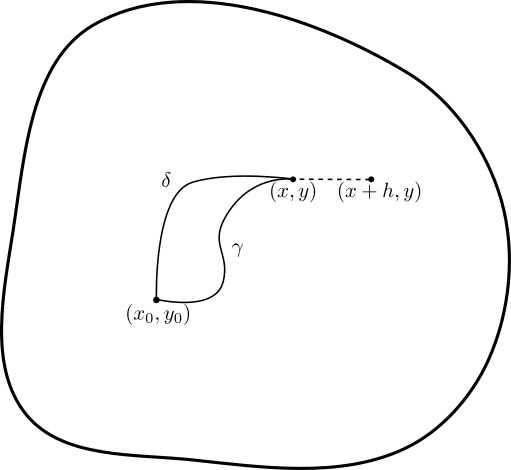
\includegraphics[scale=0.9]{Images/primitive_existence.png}
        \caption{Define primitives by integrating along paths}
        \label{fig:primitive-existence}
    \end{figure}    
    
    Suppose $\omega = Pdx + Qdy$. We want to show that the partial derivatives of $F$ are $P$ and $Q$. In order to compute $\frac{\partial F}{\partial x}$, we need to compute the difference $F(x + h, y) - F(x, y)$. I claim that
    $$ F(x + h, y) - F(x, y) = \int_{x}^{x+h} P(t, y) dt $$
    We can see this by choosing our paths cleverly.
    In order to compute $F(x + h, y)$ we need a path from $(x_0, y_0)$ to $(x + h, y)$. The path we will choose will go to $(x, y)$ first and then go to $(x + h, y)$ on a horizontal path $\sigma$. Then
    \begin{align*}
        F(x + h, y) - F(x, y) &= \int_{\gamma * \sigma} \omega - \int_{\gamma} \omega\\
        &= \int_{\sigma} \omega \\
        &= \int_{0}^1 \sigma^*(P dx + Q dy)\\
        &= \int_{0}^1 (P \circ \sigma) d(x \circ \sigma) + \int_0^1 (Q \circ \sigma) d(y \circ \sigma)\\
        &= \int_{x}^{x + h} P(t, y) dt 
    \end{align*}
    where in the final equality we use the fact that $d(y \circ \sigma) = 0$ since $\sigma$ is constant in the $y$-direction and do a substitution for the first coordinate (namely we have $z = \sigma(x)$).
    
    Then 
    $$ \frac{\partial}{\partial x} F(x, y) = \lim_{h \to 0} \frac{F(x + h, y) - F(x, y)}{h} = \lim_{h \to 0} \frac{1}{h} \int_x^{x + h} P(t, y) dt = P(x, y) $$
    where the final equality comes from the Fundamental Theorem of Calculus. We can similarly conclude $\frac{\partial }{\partial y}F(x, y) = Q$ giving us the desired result.
\end{proof}